% A0 scientific poster (portrait) -- IE Research Capstone, Marco Ortiz Togashi.
% Reuses the thesis figures (figures/*.pdf) and palette. Compile: pdflatex poster_a0.tex
\documentclass[25pt, a0paper, portrait, margin=12mm, innermargin=16mm,
               blockverticalspace=16mm, colspace=16mm, subcolspace=8mm]{tikzposter}

\usepackage[T1]{fontenc}
\usepackage{amsmath,amssymb}
\let\Bbbk\relax            % avoid amssymb/newtxmath clash on \Bbbk
\usepackage{newtxtext,newtxmath}
\usepackage{graphicx}
\usepackage[export]{adjustbox}
\usetikzlibrary{calc}
\usepackage{enumitem}
\setlist[itemize]{leftmargin=1.4em, itemsep=2pt, topsep=3pt}
\usepackage[document]{ragged2e}   % ragged-right body kills justification rivers
\setlength{\parskip}{6pt}          % internal air between paragraphs

\definecolor{navy}{HTML}{1F3B63}
\definecolor{gold}{HTML}{E69F00}
\definecolor{rust}{HTML}{B3402F}
\definecolor{sage}{HTML}{4A7C59}
\definecolor{paper}{HTML}{F7F7F4}
\colorlet{navylt}{navy!8}      % pre-mixed (xcolor expressions fail inside coloredbox opts)
\colorlet{goldlt}{gold!18}
\colorlet{navytint}{navy!9}    % faint hero panel tint

% Fixed safe content width for the full-bleed-prone hero/spine bands (printable area).
\newlength{\spinew}\setlength{\spinew}{1750pt}
\newlength{\spineshift}\setlength{\spineshift}{-173pt}

% The ONE repeating motif: a 2.5pt meaning-coded accent rule under each block title.
\newcommand{\accentrule}[1][navy]{\par\vspace{-3mm}{\color{#1}\rule{\linewidth}{2.5pt}}\par\vspace{2mm}}

%, theme + Johns-Hopkins-style flat blocks (centered navy header bar, borderless body) ,
\usetheme{Default}
\usecolorstyle{Germany}
\colorlet{titlefgcolor}{white}
\colorlet{titlebgcolor}{navy}
\colorlet{blocktitlebgcolor}{navy}
\colorlet{blocktitlefgcolor}{white}
\colorlet{backgroundcolor}{white}
\colorlet{framecolor}{white}
\colorlet{notefgcolor}{black}
\colorlet{notebgcolor}{gold!25}

% Flat, conference-poster block: a centered filled navy title bar, no body frame.
\defineblockstyle{JHbar}{
  titlewidthscale=1, bodywidthscale=1,
  titleoffsetx=0pt, titleoffsety=0pt, bodyoffsetx=0pt, bodyoffsety=0pt,
  bodyverticalshift=2mm, roundedcorners=5, linewidth=0pt,
  titleinnersep=6mm, bodyinnersep=2mm
}{
  \ifBlockHasTitle
    \draw[draw=none, fill=blocktitlebgcolor, rounded corners=\blockroundedcorners]
      (blocktitle.south west) rectangle (blocktitle.north east);
  \fi
  % body intentionally undrawn -> content flows flat on the white background
}
\useblockstyle{JHbar}
\settitle{
  % === conference-poster title bar: IE logo left, title centered ===
  \begin{minipage}[c]{0.17\linewidth}\centering
    \IfFileExists{../figures/ie_logo.pdf}{%
      {\setlength{\fboxsep}{6mm}\colorbox{white}{
\includegraphics[height=3.4cm]{../figures/ie_logo.pdf}}}}{%
      \IfFileExists{../figures/ie_logo.png}{%
        {\setlength{\fboxsep}{6mm}\colorbox{white}{
\includegraphics[height=3.4cm]{../figures/ie_logo.png}}}}{%
        {\color{titlefgcolor}\large IE University\\[2pt]School of Sci.\ \& Tech.}}}
  \end{minipage}\hfill
  \begin{minipage}[c]{0.80\linewidth}\centering
    {\color{titlefgcolor}\bfseries\fontsize{46}{54}\selectfont
     Does Spatial Correlation of Carbon Intensity Improve\\[4pt]
     Robust Carbon-Aware Data-Center Scheduling?\par}
    \vspace{0.3cm}
    {\color{titlefgcolor}\Large
     A Multi-Grid Falsification Study: Causal Mechanism, Copula Test, and an Active-Transfer Extension\par}
    \vspace{0.3cm}
    {\color{titlefgcolor}\normalsize \textbf{Marco Ortiz Togashi}\quad$\cdot$\quad
     Supervisor: Prof.\ Bissan Ghaddar\quad$\cdot$\quad
     IE University, Master in Business Analytics \& Data Science\par}
  \end{minipage}
}
\title{Carbon DRO}  % placeholder; the real title is hardcoded in \settitle above
\tikzposterlatexaffectionproofoff   % remove default bottom-right watermark

\begin{document}
\maketitle

% ===================== HERO BANNER (full width) =====================
\begin{columns}
\column{1}
\block{}{%
  \noindent\hspace*{\spineshift}%
  \setlength{\fboxsep}{0pt}\colorbox{navytint}{\parbox{\spinew}{%
  \vspace{6mm}\par\noindent
  {\color{gold}\rule{\linewidth}{2pt}}\\[5mm]
  \noindent
  \begin{minipage}[c]{0.605\linewidth}\centering
    \vspace{2mm}
    \begin{tikzpicture}
      \node[inner sep=0] (img)
        {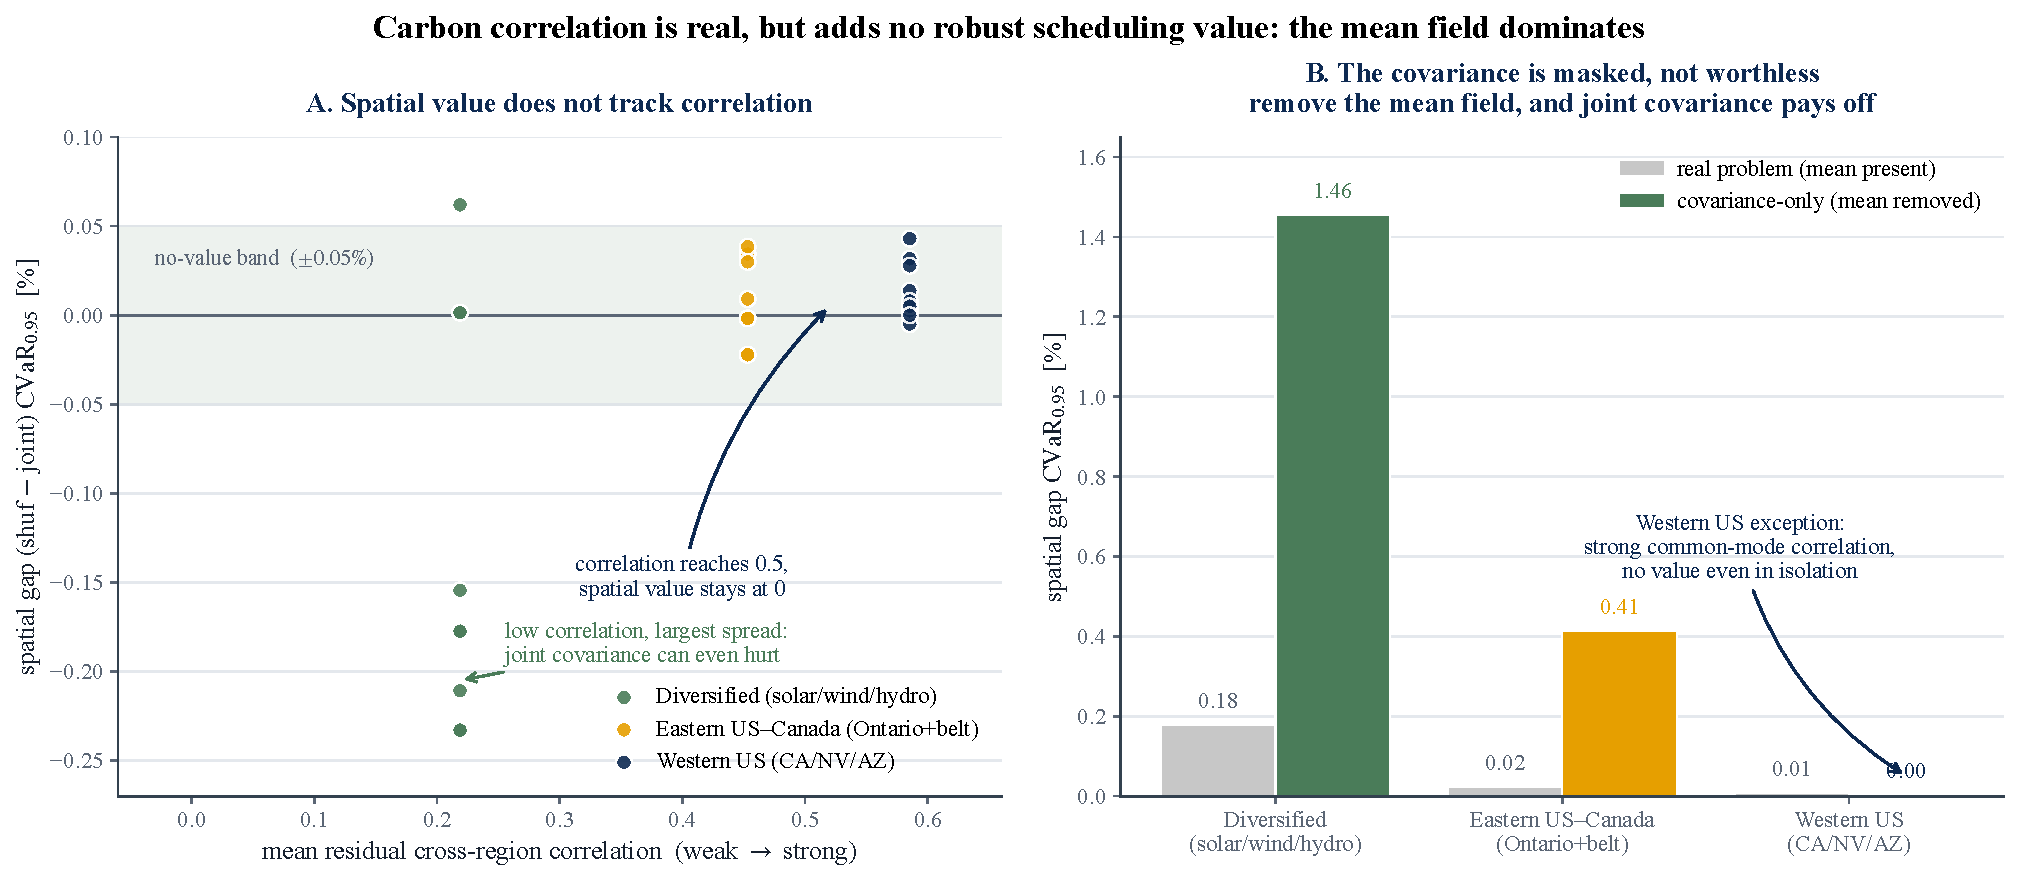
\includegraphics[height=22cm,trim={0bp 0bp 463bp 40bp},clip]{../figures/finding.pdf}};
      \draw[gold,line width=3pt,opacity=0.92]
        ([yshift=0pt]$(img.south west)!0.705!(img.north west)$) --
        ([yshift=0pt]$(img.south east)!0.705!(img.north east)$);
    \end{tikzpicture}
    \vspace{2mm}
  \end{minipage}\hfill
  \begin{minipage}[c]{0.355\linewidth}\RaggedRight
    {\bfseries\color{navy}\fontsize{33}{39}\selectfont
     Across every grid and every model, the gap never leaves {\color{gold}zero}.}\\[5mm]
    {\color{gold}\rule{0.92\linewidth}{2.5pt}}\\[4mm]
    {\color{navy}\fontsize{21}{26}\selectfont
     The diurnal \textbf{\color{rust}mean} carbon field, not its spatial \textbf{shape}, is what a robust scheduler can act on.}
  \end{minipage}%
  \par\vspace{6mm}}}%
}
\end{columns}
\vspace{8mm}

% ===================== ANSWER SPINE (full width, reads in 5s from 3m) =====================
\begin{columns}
\column{1}
\block{}{%
  \newcommand{\spinecell}[3]{%
    \begin{minipage}[c]{0.235\spinew}\centering
      {\bfseries\fontsize{68}{72}\selectfont\color{#1} #2}\\[1mm]
      {\color{navy}\scshape\fontsize{18}{22}\selectfont #3}
    \end{minipage}}%
  \noindent\hspace*{\spineshift}%
  \setlength{\fboxsep}{0pt}\colorbox{navytint}{\parbox{\spinew}{\vspace{7mm}\par\noindent
  \spinecell{navy}{$0.78$}{cross-grid correlation\\is real}\hfill
  \textcolor{navy!30}{\rule[-2.4cm]{1.4pt}{4.8cm}}\hfill
  \spinecell{gold}{$\sim$0\%}{robust scheduling\\value}\hfill
  \textcolor{navy!30}{\rule[-2.4cm]{1.4pt}{4.8cm}}\hfill
  \spinecell{rust}{$+1.46\%$}{only when the\\mean is flattened}\hfill
  \textcolor{navy!30}{\rule[-2.4cm]{1.4pt}{4.8cm}}\hfill
  \spinecell{sage}{4-10\%}{only via\\active transfer}%
  \par\vspace{7mm}}}%
}
\end{columns}
\vspace{6mm}

% ===================== NULL-PROOF STRIP (schedule overlay) =====================
\begin{columns}
\column{1}
\block{}{%
  \noindent\hspace*{\spineshift}%
  \begin{minipage}{\spinew}\centering
    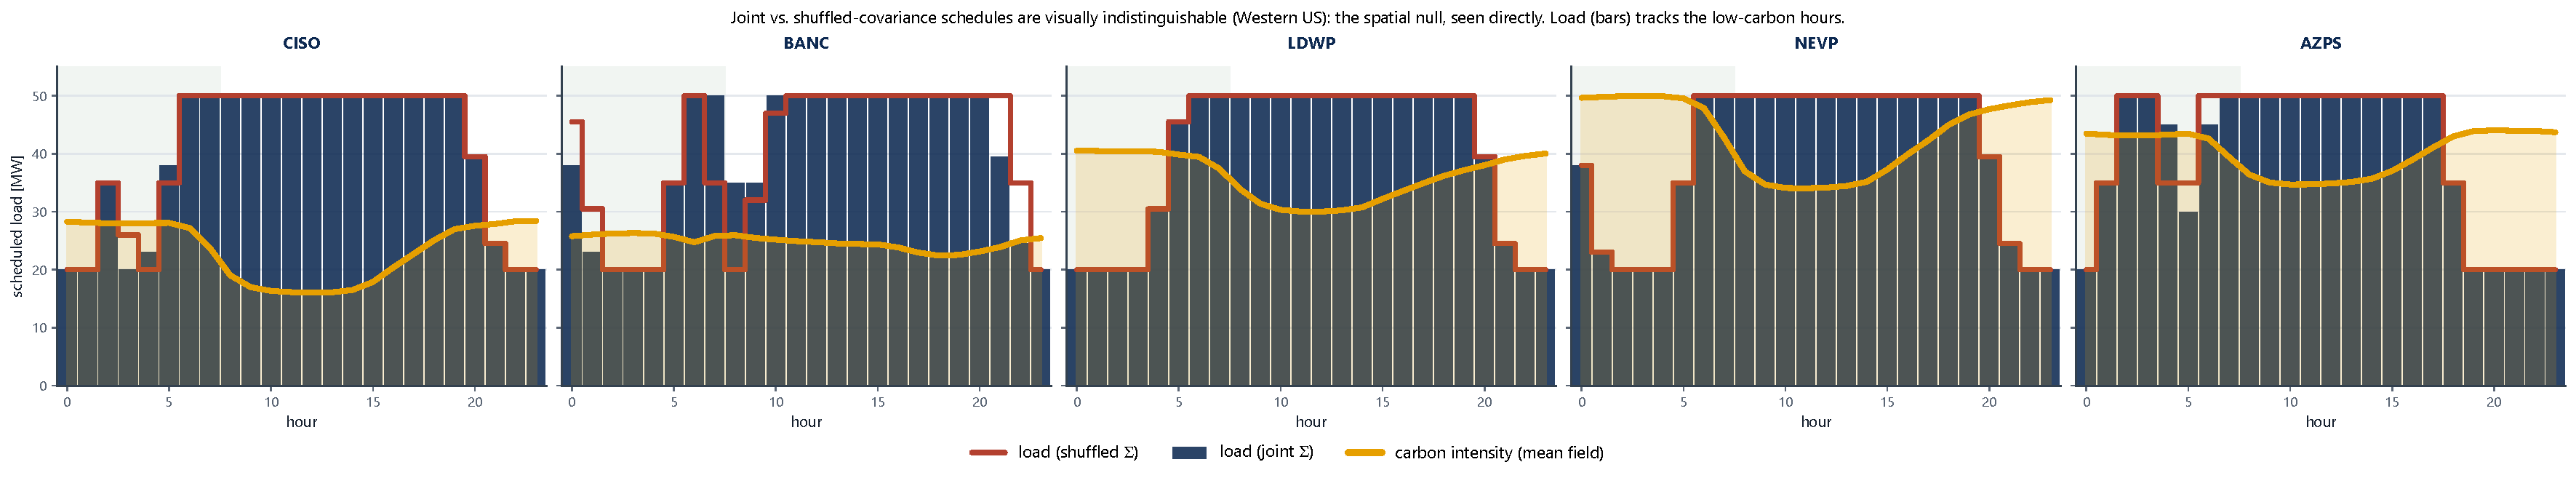
\includegraphics[width=\linewidth]{../figures/schedule_us_west.pdf}
  \end{minipage}%
}
\end{columns}
\vspace{10mm}

\begin{columns}

% ===================== COLUMN 1 =====================
\column{0.33}

\block{The setup}{
\accentrule[navy]
\begin{itemize}
\item Data centers consume 1--2\% of global electricity, and compute is unusually
\textbf{flexible}: batch/training jobs can shift in time and across sites.
\item Carbon intensity varies strongly by hour and region, so a scheduler can defer
work to cleaner moments.
\item Robust scheduling under \emph{uncertain} carbon intensity uses
\textbf{distributionally robust optimization (DRO)}.
\item A natural extension treats carbon intensity as a stochastic \emph{vector} so
that \textbf{spatial correlation} can inform the schedule.
\end{itemize}
\vspace{0.3cm}
\coloredbox[bgcolor=navylt, framecolor=navy]{
\textbf{RQ1.} Is carbon intensity of coupled grids genuinely correlated?\\[2pt]
\textbf{RQ2.} Does feeding that correlation to a covariance-based DRO reduce
out-of-sample tail emissions ($\mathrm{CVaR}_{0.95}$)?\\[2pt]
\textbf{RQ3.} If not, \emph{why}, and what dependence structure would a richer
model need?
}
}

\block{How we test it}{
\accentrule[navy]
A Mahalanobis--Wasserstein DRO, solved as a second-order cone program:
\vspace{-0.2cm}
{\small\[
\min_{x\in\mathcal X,\,t\ge0}\ \langle\bar\rho,x\rangle+\varepsilon\,t
\quad\text{s.t.}\quad \lVert L^\top\!\mathrm{vec}(x)\rVert_2\le t,\ \ LL^\top=\hat\Sigma .
\]}
\textbf{Shuffled-marginals test.}
\begin{itemize}
\item Fit the schedule twice, on the \emph{joint} covariance vs.\ a
\emph{block-diagonal} one with all cross-region structure zeroed, and compare
out-of-sample $\mathrm{CVaR}_{0.95}$ of daily emissions.
\item The \emph{spatial gap} is positive iff the joint covariance helps.
\end{itemize}
\begin{itemize}
\item Pre-registered: config commit-locked, single 2025 test read.
\item Five region sets: 3 US/Canada grids spanning low-to-strong correlation
($\bar r\!\approx\!0.2$ to $0.65$) $+$ a near-zero Iberia--France anchor.
\item Blocked 5-fold CV selects $\varepsilon^\star$; 1000-bootstrap CIs.
\end{itemize}
}

\block{Correlation is real}{
\accentrule[navy]
After removing each zone's hour-of-day mean, residual cross-region correlation is
\textbf{strong and survives de-seasonalization}: US West CISO--NEVP
$\textcolor{navy}{\mathbf{0.78}}$; Ontario belt CA-ON--NYISO
$\textcolor{navy}{\mathbf{0.73}}$. The three grids and their correlation network:
\vspace{0.4cm}
\par\vspace{0.25cm}
\begin{center}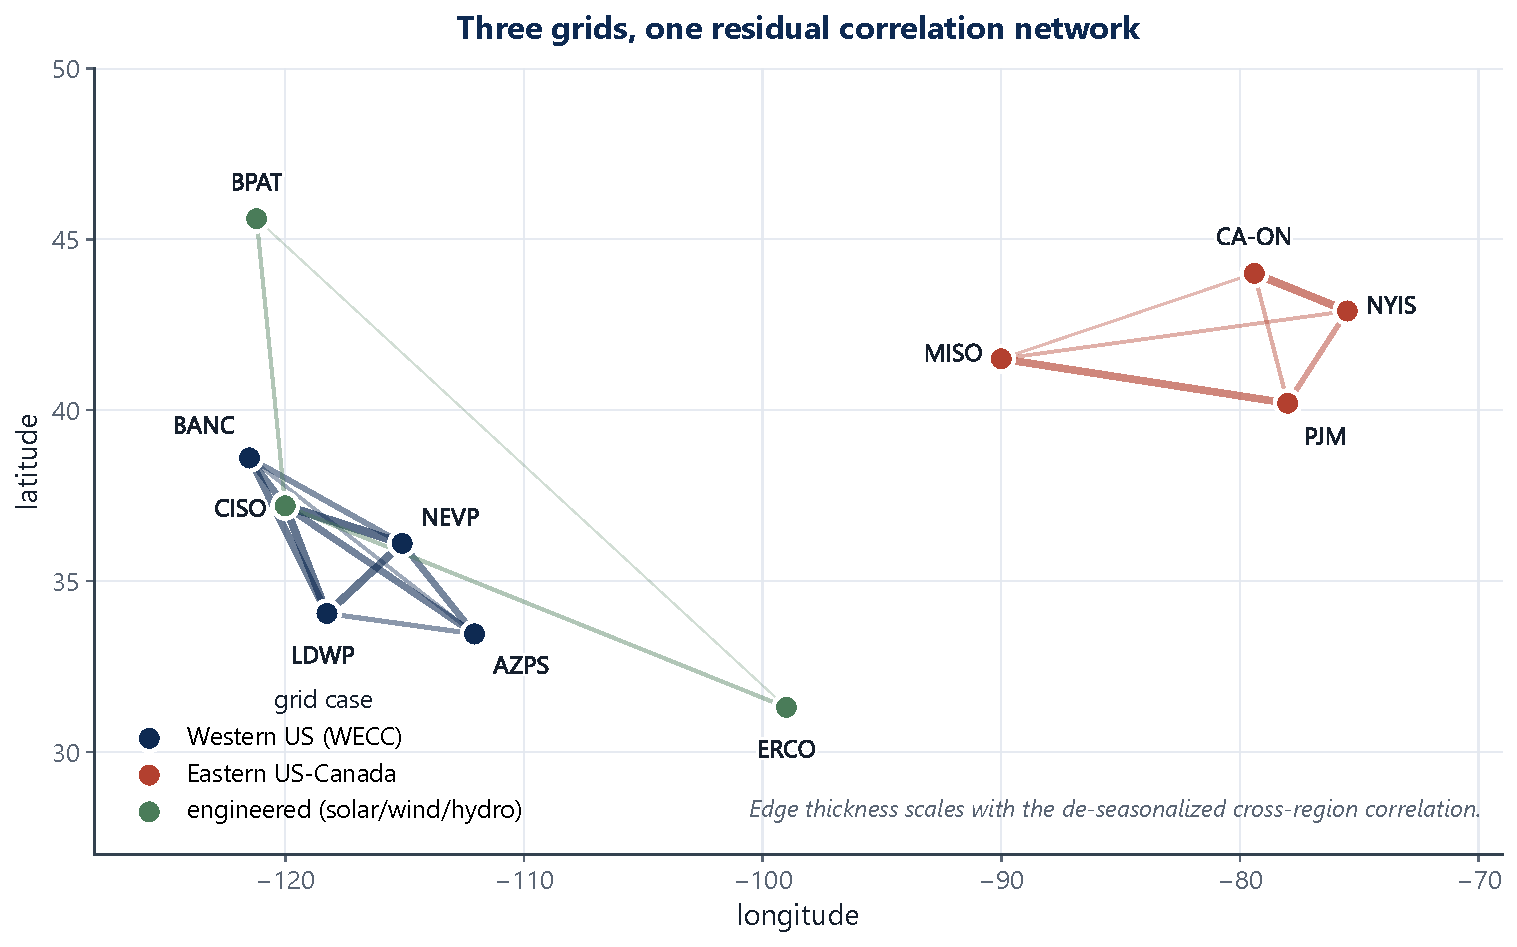
\includegraphics[width=0.92\linewidth]{../figures/correlation_map.pdf}\end{center}
\vspace{0.2cm}
\innerblock{}{\centering\textbf{The assumption motivating spatial DRO is empirically
valid.}}
}

% ===================== COLUMN 2 =====================
\column{0.34}

{\colorlet{blocktitlebgcolor}{gold!88!navy}
\block{Value is zero}{
\accentrule[gold]
The spatial gap is not merely small, it is \emph{certified} zero across the whole
dependence spectrum:
\begin{itemize}
\item Survives Ledoit--Wolf shrinkage, seasonal/AR(1) residualization, and the full
tail range $\mathrm{CVaR}_{0.90}$ to $\mathrm{CVaR}_{0.99}$.
\item Survives Benjamini--Hochberg correction over 144 cells and walk-forward
testing to 2024.
\item A per-cell \textbf{equivalence test (TOST)} affirmatively rejects any effect
above the $\textcolor{gold}{\textbf{0.4\%}}$ materiality margin in all $27$ cells.
\item The gap is statistically $\textcolor{gold}{\mathbf{=0}}$, not merely undetected.
\end{itemize}
\innerblock{}{This is an \textbf{active null}: CV selects $\varepsilon^\star=1$ in
nearly every cell, so the DRO is genuinely robustifying, and the covariance
\emph{still} buys nothing.}
}}

{\colorlet{blocktitlebgcolor}{rust!82!navy}
\block{The mean is the cause}{
\accentrule[rust]
\begin{itemize}
\item \textbf{Mean-ablation (causal).} Flatten the mean carbon field and the joint
covariance suddenly pays, up to $\textcolor{rust}{\mathbf{+1.46\%}}$. The spatial
signal is \textbf{real but masked} by the diurnal mean field, not absent.
\item \textbf{Tail dependence (structural).} The residual dependence is
\textbf{non-elliptical}: regions go \emph{clean} together more than \emph{dirty}
together ($\chi_L>\chi_U$, upper-tail independent). An elliptical covariance ball
forces $\chi_L=\chi_U$, it is the \emph{wrong object}.
\end{itemize}
\vspace{0.45cm}
\begin{center}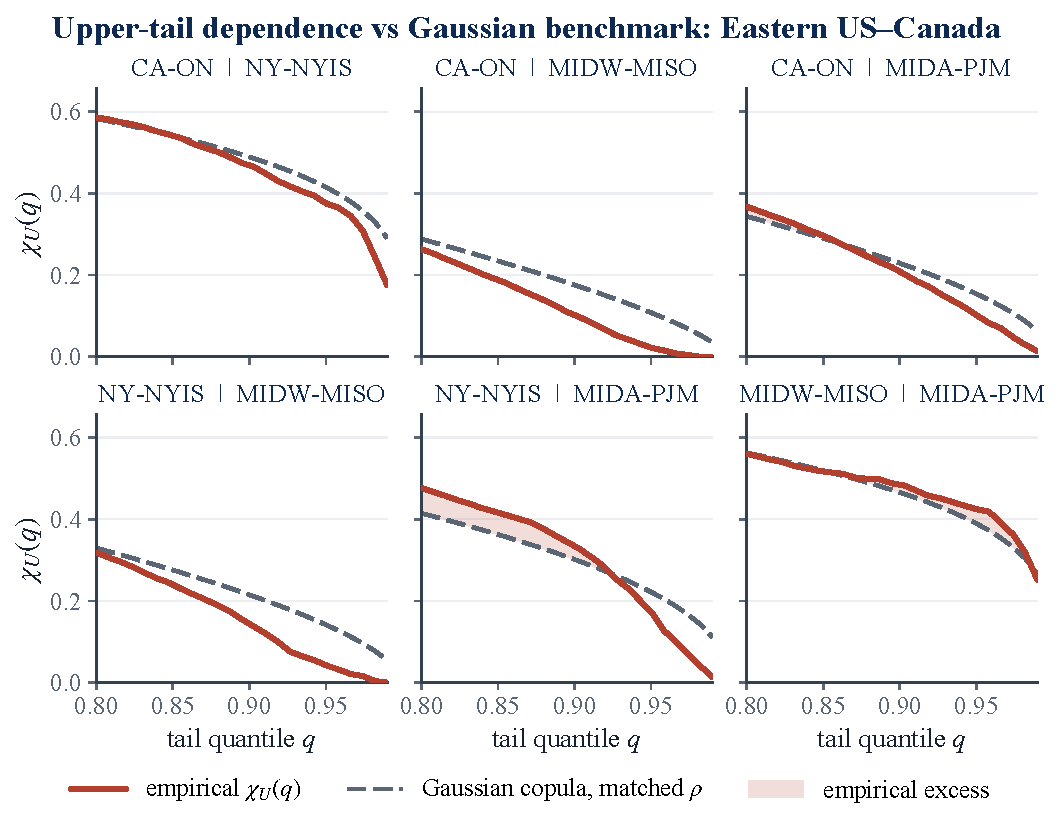
\includegraphics[width=0.9\linewidth]{../figures/tail_dependence_taskc.pdf}\end{center}
}}

% ===================== COLUMN 3 =====================
\column{0.33}

\block{Even the right copula fails}{
\accentrule[rust]
We replace the covariance ball with copula schedulers (CVaR sample-average) that
\emph{can} represent the asymmetry: independence, Gaussian, lower-tail
\textbf{Clayton}, and the maximal \textbf{comonotone} (upper Fr\'echet $\sup_C$).
\par\vspace{0.35cm}
\begin{center}
\begin{minipage}{0.46\linewidth}\centering
  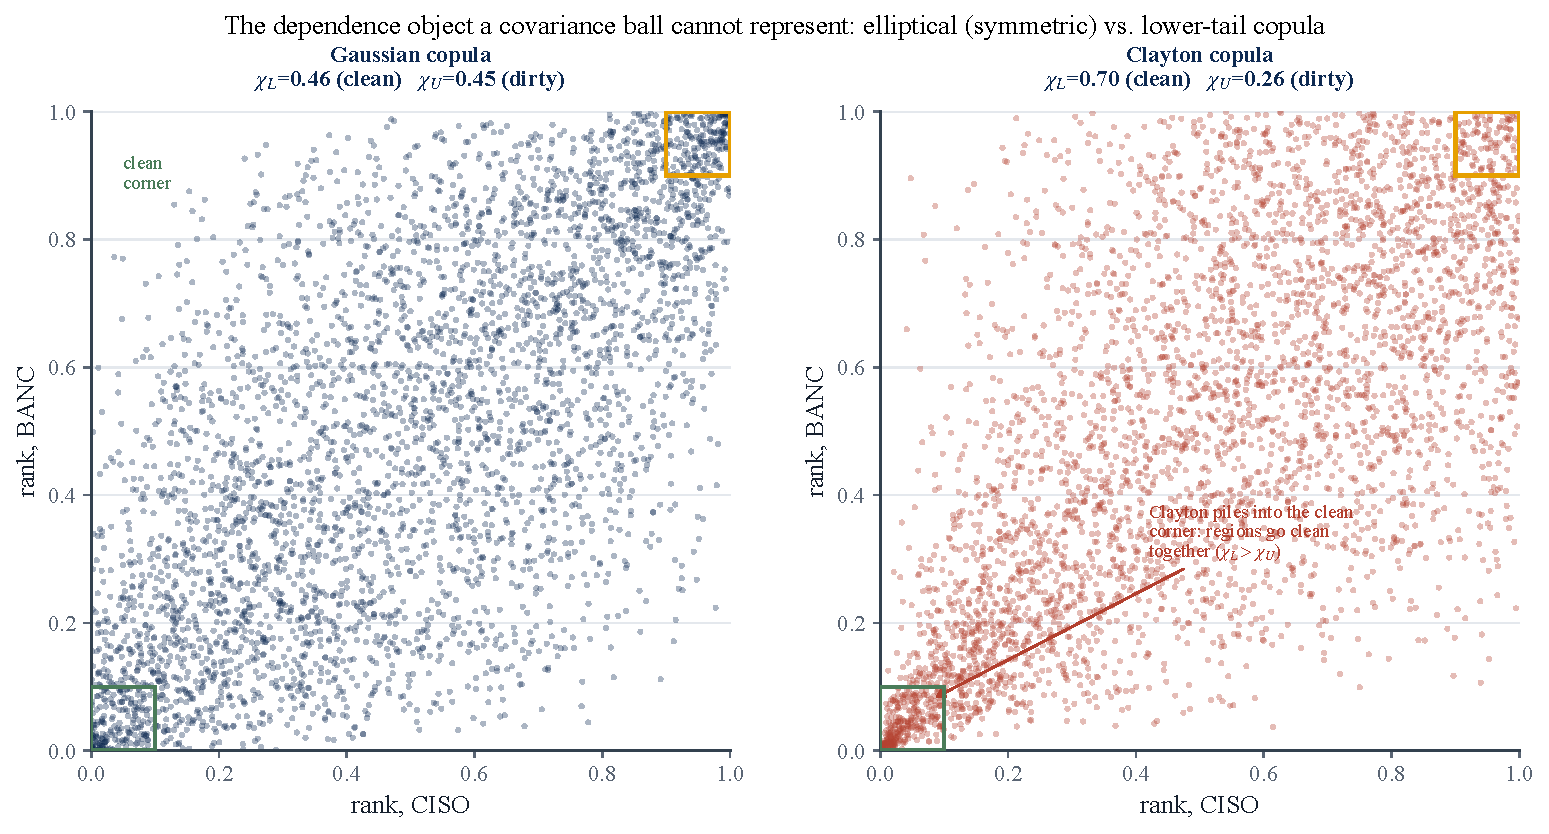
\includegraphics[width=\linewidth]{../figures/copula_density.pdf}
\end{minipage}\hfill
\begin{minipage}{0.46\linewidth}\centering
  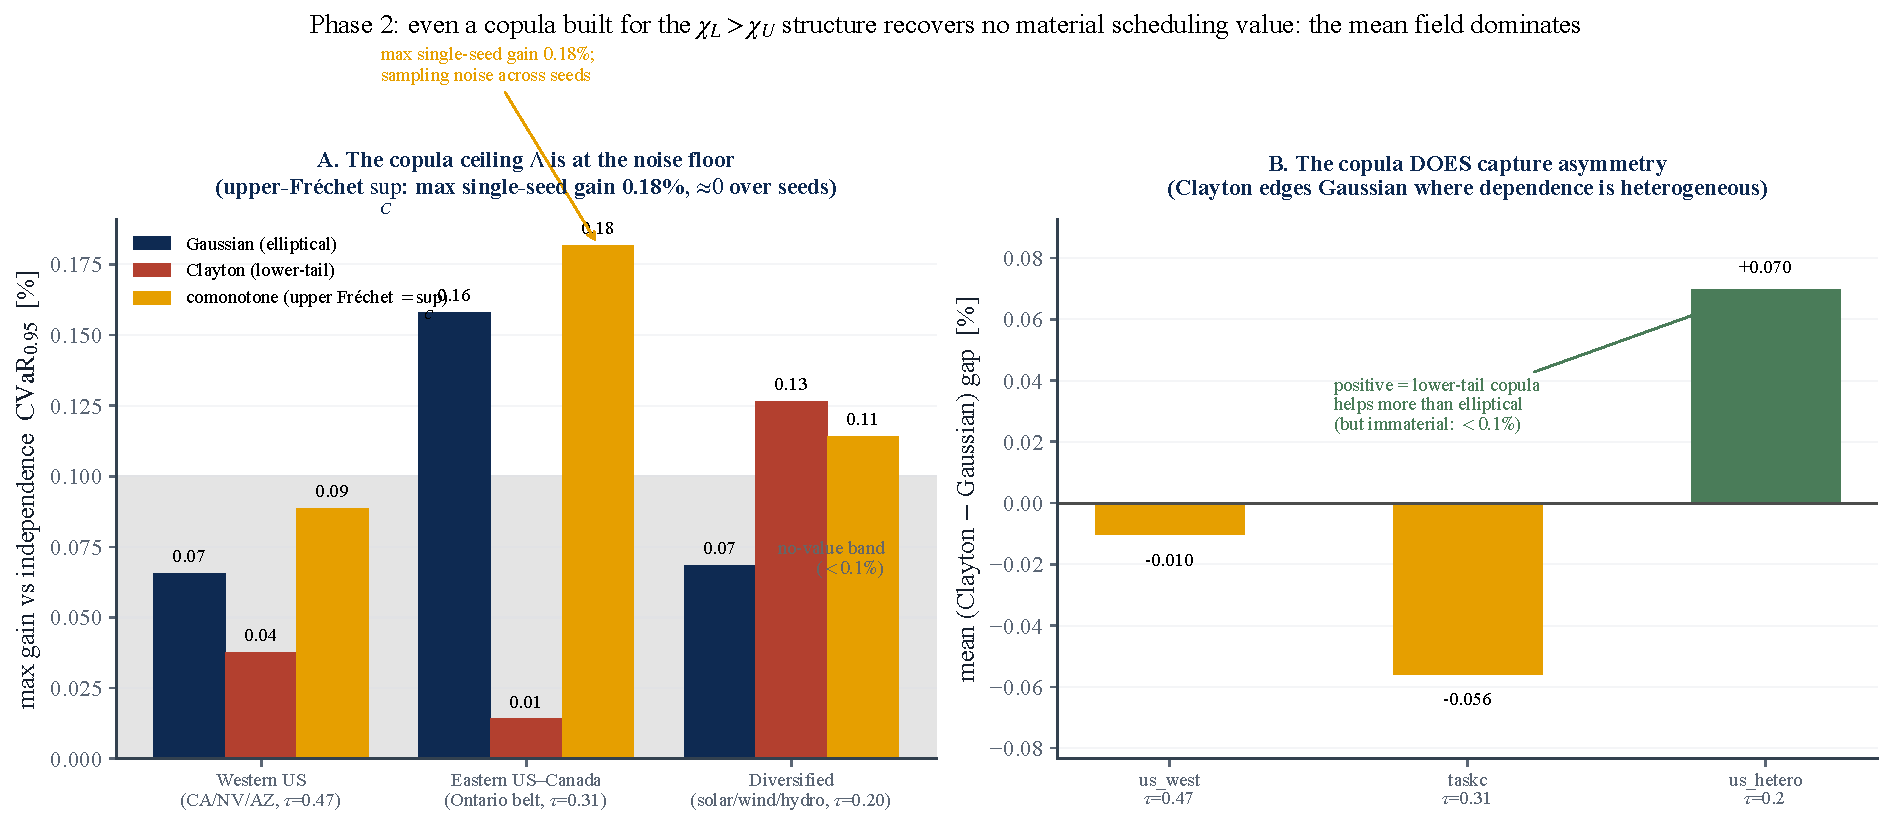
\includegraphics[width=\linewidth]{../figures/copula_result.pdf}
\end{minipage}
\end{center}
\vspace{0.3cm}
\innerblock{}{Even the \emph{maximal} copula's gain sits at the scenario-noise
floor ($|\Lambda|\lesssim\mathbf{0.1\%}$, $\approx0$ over seeds): the null is
\textbf{total}.}
}

\block{A mean-dominance bound}{
\accentrule[navy]
By translation invariance of CVaR, $\langle\rho,x\rangle=\langle\bar\rho,x\rangle
+\langle\xi,x\rangle$, the dependence model moves only the residual term.
\vspace{0.15cm}
\coloredbox[bgcolor=goldlt, framecolor=rust]{
\textbf{Proposition.} For the SOCP, the spatial gap obeys
$\big|\mathrm{OPT}(\Sigma)-\mathrm{OPT}(\Sigma^{\mathrm{shuf}})\big|\le
\varepsilon\,(\max_{x}\lVert x\rVert_2)\,\lVert\Sigma^{\mathrm{off}}\rVert_2^{1/2}$,
vanishing as $\varepsilon\to0$ or $\Sigma^{\mathrm{off}}\to0$.}
\vspace{0.15cm}
The tight ceiling is \emph{measured} by the comonotone arm
($|\Lambda|\!\lesssim\!0.1\%$, at the scenario-noise floor), an order below the
mean-driven value.
}

{\colorlet{blocktitlebgcolor}{sage!85!navy}
\block{We built the one open route}{
\accentrule[sage]
\begin{itemize}
\item Spatial correlation of carbon is \textbf{real but adds no robust scheduling
value}, anywhere on the spectrum, for \emph{any} passive dependence model.
\item The binding constraint is the \textbf{mean field}, not the shape of the
dependence (mean-dominance bound $+$ comonotone ceiling).
\item \textbf{Recommendation:} per-region marginal schedulers capture essentially
all the value at a fraction of the cost.
\item \textbf{We built the one route the bound leaves open}, an \emph{active}
inter-region transfer channel $f_{r\to s,t}$. It cuts
\textcolor{sage}{\textbf{4-10\%}} \emph{deterministically} by exploiting the
spatial mean.
\item But \emph{robustifying} it pays nowhere data-grounded, online or under real
tail-day emergencies. The null extends to the active and online settings: value
lives in the decision, not the dependence model.
\end{itemize}
\vspace{0.35cm}
{\color{sage}\rule{\linewidth}{2.5pt}}\par\vspace{2mm}
{\footnotesize Reproducible pipeline: \textbf{187 unit tests}, pre-registered configs,
  per-cell equivalence tests, multi-seed stability, an independent adversarial
  review, license-safe archived results. \emph{AI used as a coding/drafting
  assistant under the author's direction.}\par}
}}

\end{columns}
\end{document}
